\section{Numerical Results} \label{result}

To study the numerical accuracy and efficiency of the methods above, in this section, we present the numerical results for the Laplace equations, the reaction-diffusion equations, and the Stokes equations in an irregular domain. The bounding box $\mathcal{B}$ embedding the domain $\Omega$ for solving the interface problem is specified as a square(cube), whose size as well as the curve(surface) parameters are given respectively in the description of each numerical example.

The following examples give the convergent error of the numerical discretization scheme. Taking two dimensions as an example, the error is defined as $e_{i j}$ with $e_{i j}=\left(u_h\right)_{i j}-\left(u^*\right)_{i j}$, where $N$ is the number of interior grid nodes, $u^*$ is the exact solution, $u_h$ is the numerical solution with step size $h$. Denote by $\left\|\mathrm{e}_h\right\|_{\infty}$ and $\left\|\mathrm{e}_h\right\|_2$ the discrete maximum norm and the scaled discrete $l_2$-norm of $e_{i j}$ respectively, i.e.,
$$
\begin{aligned}
\left\|\mathbf{e}_h\right\|_{\infty} & =\max _{\left(x_i, y_j\right) \in \Omega}\left|e_{i j}\right| \\
\left\|\mathbf{e}_h\right\|_2 & =\sqrt{\frac{1}{N} \sum_{\left(x_i, y_j\right) \in \Omega}\left|e_{i j}\right|^2}
\end{aligned}
$$

To check the algorithm's accuracy, we verify the numerical error in each case with the grid refinement. The GMRES iteration stops when the iterated residual in the discrete $\ell^2$-norm relative to that of the initial residual is less than a prescribed tolerance and is fixed to be $10^{-8}$. The corresponding table for each case lists the step size, the number of grid points, the CPU times, the GPU times, and the speedup ratios. Numerical results on the Cartesian grid to the problem are also displayed in the plots for each fixed time.

In addition, we perform numerical experiments on eight NVIDIA GeForce RTX 3090 graphics cards, which contain 10496 cores organized in 84 streaming multiprocessors (MPs). Moreover, it provides 24GB of device memory with a memory bandwidth of 936GB/s, accessible by all its cores and the CPU through the Intel(R) Xeon(R) Gold 6330 CPU with 28 cores.

\begin{table}[H]
\centering
\begin{tabular}{c|c|ccccc}
\hline Poisson & \text { grid size }  & $512^2$ & $1024^2$ & $2048^2$ &  $4096^2$\\
\hline FFT
 & GPU time & $0.19 \mathrm{~s}$ & $0.27 \mathrm{~s}$ & $0.66 \mathrm{~s}$ & $1.65\mathrm{~s}$  \\
\hline Multigrid&  GPU time & $0.25 \mathrm{~s}$ & $0.61 \mathrm{~s}$ & $2.08 \mathrm{~s}$ & $8.66\mathrm{~s}$  \\
\hline
\end{tabular}
    \caption{\footnotesize{\small{Comparison of different Poisson solvers on DBVP of the Laplace equation.}}}
    \label{tab:FFTvsMultigrid}
\end{table}
\begin{table}[H]
\centering
\begin{tabular}{c|c|ccccc}
\hline Iteration & \text { grid size }  & $512^2$ & $1024^2$ & $2048^2$ &  $4096^2$\\
\hline Richardson& \text {CPU time}& $5.62 \mathrm{~s}$ & $23.11 \mathrm{~s}$ & $92.05 \mathrm{~s}$ & $380.12\mathrm{~s}$ \\
 & GPU time & $0.19 \mathrm{~s}$ & $0.27 \mathrm{~s}$ & $0.66 \mathrm{~s}$ & $1.65\mathrm{~s}$  \\
\hline GMRES&  \text {CPU time}& $1.38 \mathrm{~s}$ & $5.81 \mathrm{~s}$ & $25.92 \mathrm{~s}$ & $110.21\mathrm{~s}$ \\
 & GPU time & $0.13 \mathrm{~s}$ & $0.16 \mathrm{~s}$ & $0.18 \mathrm{~s}$ & $0.25\mathrm{~s}$  \\
 \hline BiCGSTAB&  \text {CPU time}& $1.99 \mathrm{~s}$ & $8.01 \mathrm{~s}$ & $34.47 \mathrm{~s}$ & $147.49\mathrm{~s}$ \\
 & GPU time & $0.45 \mathrm{~s}$ & $0.45 \mathrm{~s}$ & $0.63 \mathrm{~s}$ & $1.01\mathrm{~s}$  \\
\hline
\end{tabular}
    \caption{\footnotesize{Comparison of various iterative methods for solving the Dirichlet boundary value problem (DBVP) associated with the Laplace equation, with a fixed tolerance level of $1e-08$ for the Richardson, GMRES, and BiCGSTAB methods.}}
    \label{tab:iter}
\end{table}
\subsection{Single GPU results}
\textbf{Example 1.} The results presented in Tab.\,\ref{tab:FFTvsMultigrid} clearly demonstrate that, within the specified range of simulation scales, the FFT+tridiagonal Poisson solver outperforms the geometric multigrid solver in terms of efficiency. This observation is consistent with the findings reported in\cite{Gholami2016}. Analyzing the results from Tab.\,\ref{tab:iter}, it is evident that the GMRES method achieves the lowest iteration number, resulting in reduced CPU and GPU time consumption. As a result, for subsequent numerical experiments, this study adopts the parallel FFT+tridiagonal Poisson solver in combination with the GMRES method for computational purposes.


This example solves the boundary value problem of the Laplace equation on the circle domain(the parameters $r_a=1.0$, $r_b=1.0$) and the rotated star-shaped domain(the parameters $m=4.0,6.0,8.0$, $r=1.0$, $c=0.2$), with the Dirichlet boundary condition. The boundary conditions are chosen so that the exact solution reads
$$
\begin{gathered}
u(x, y)=\exp(x)\cos(y) + \exp(y)\sin(x)
\end{gathered}
$$

The bounding box $\mathcal{B}$ for the interface problem is set to be $\mathcal{B}=(-1.2,1.2) \times(-1.2,1.2)$. Numerical results are plotted in Fig.\,\ref{One_Poisson1}.
\begin{figure}[htpt!]
    \centering{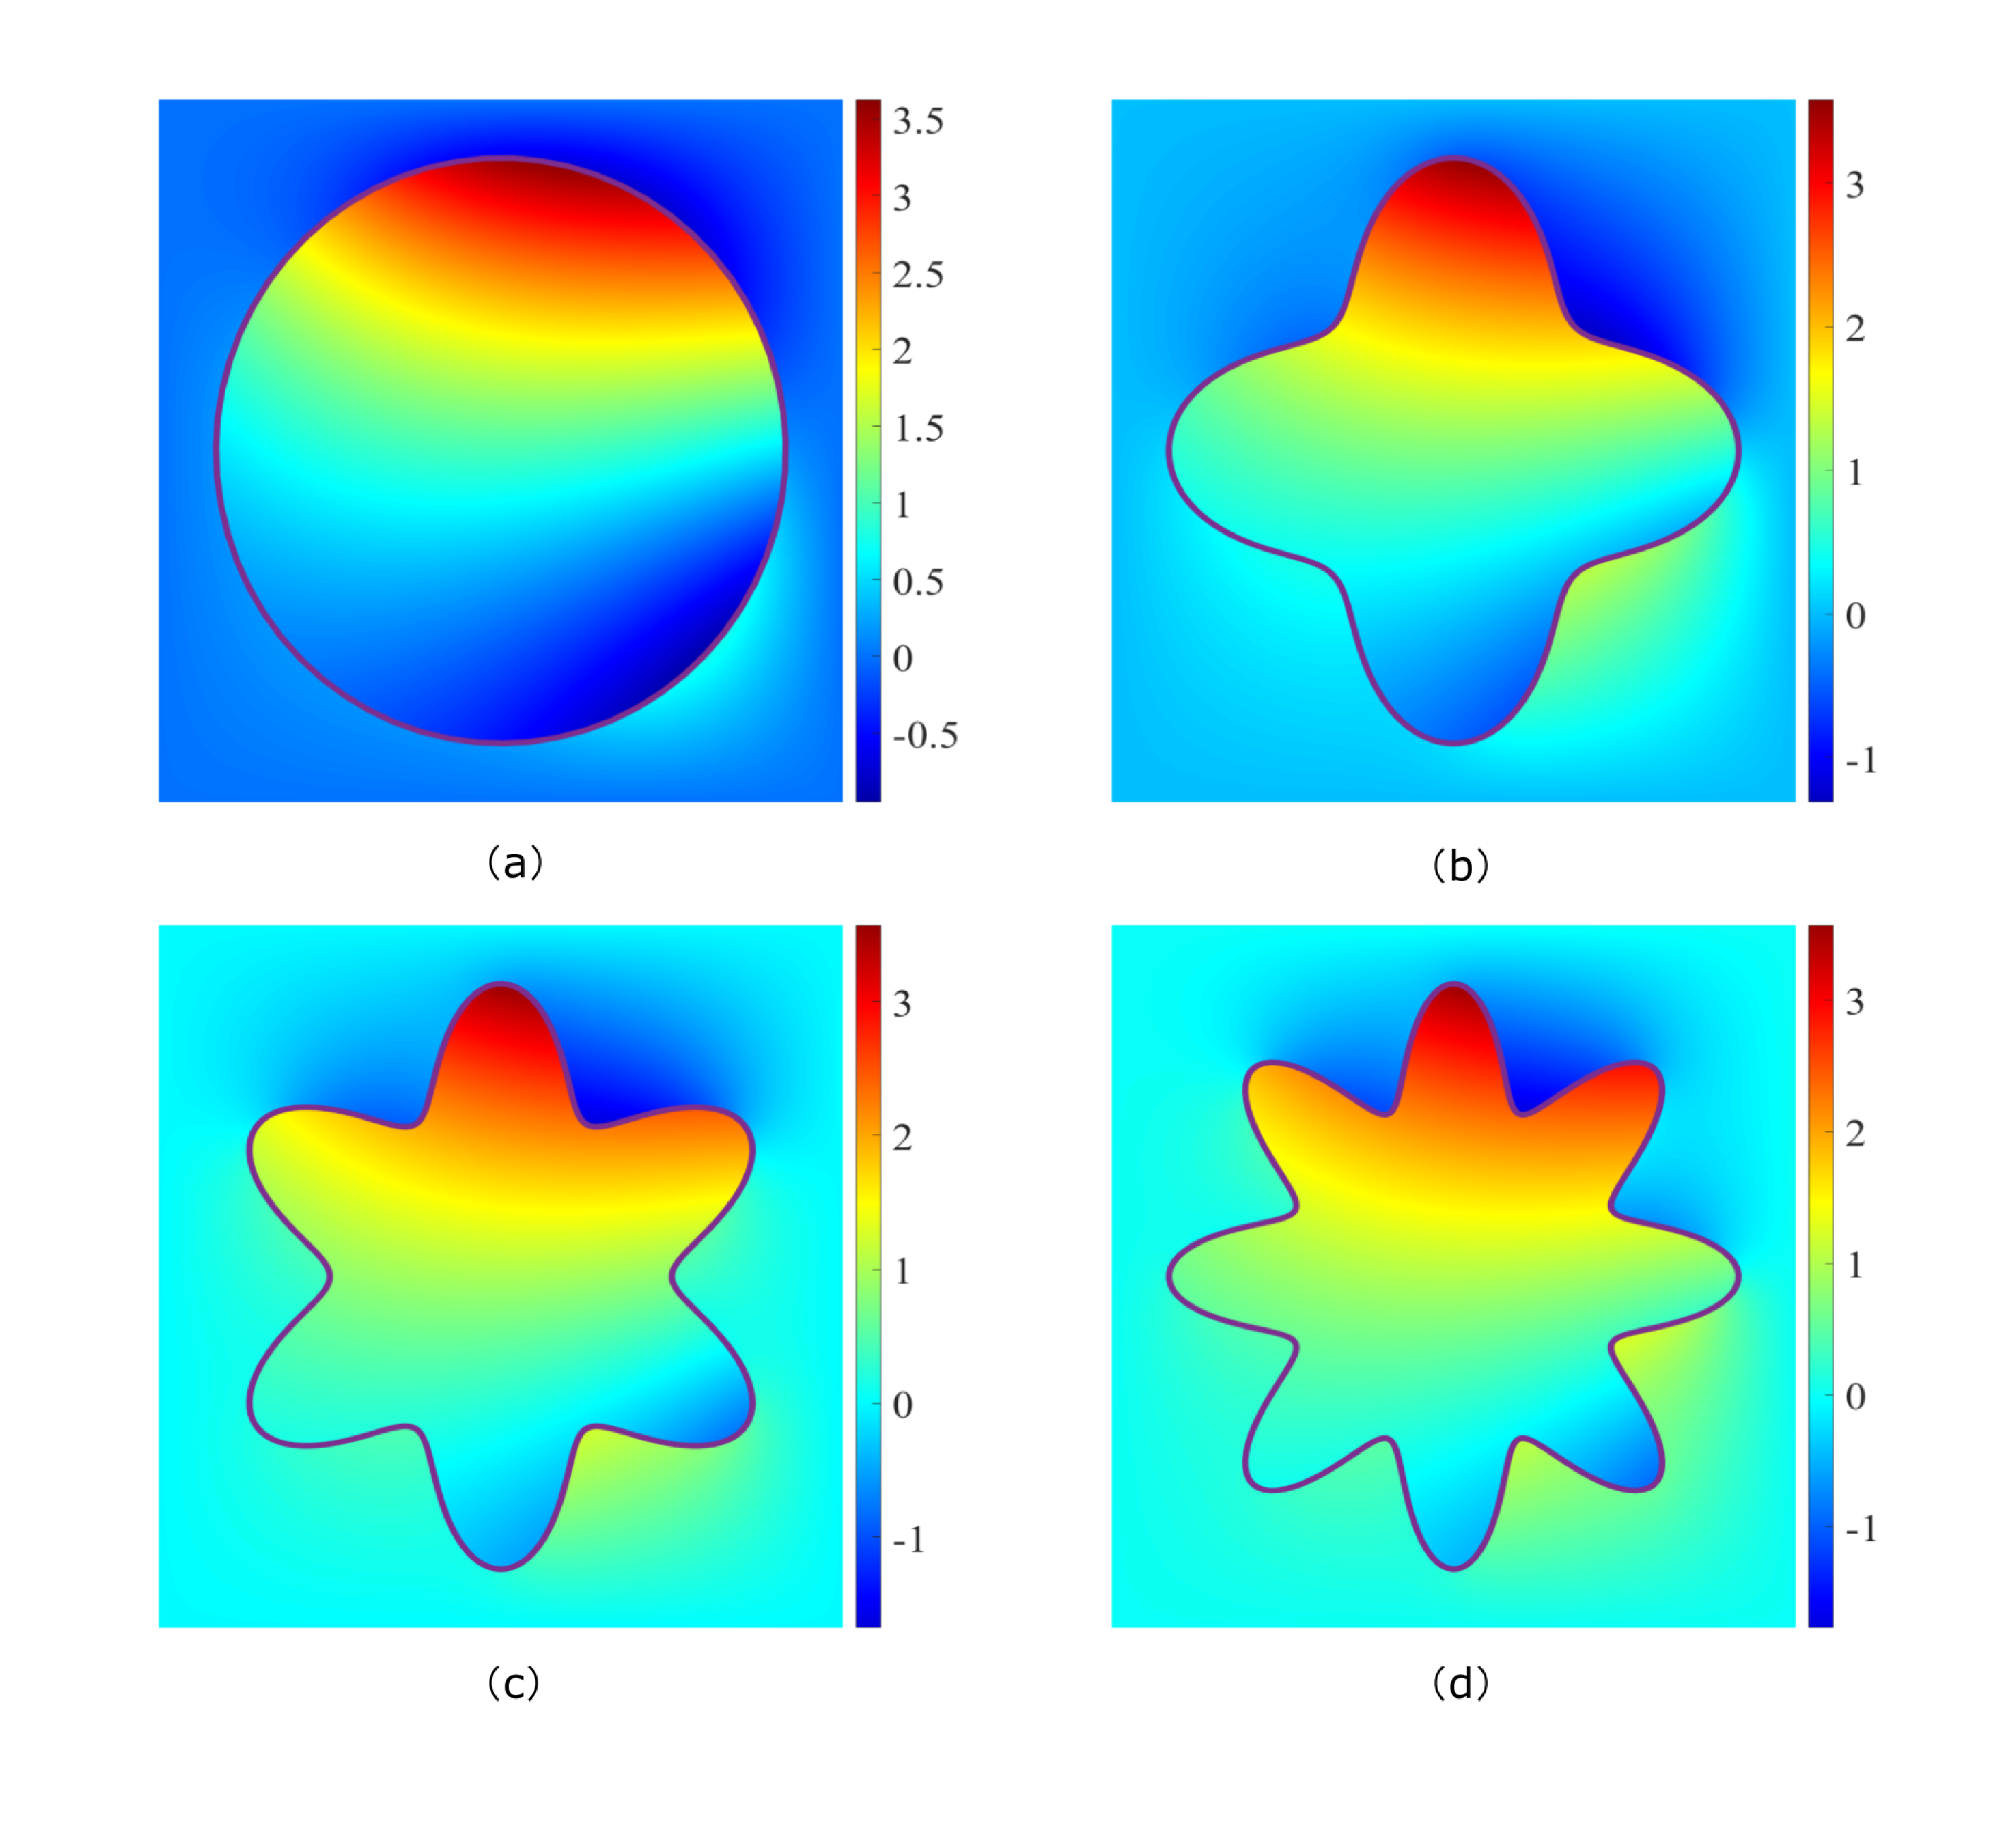
\includegraphics[width=0.6\textwidth]{figure/PNcompare1.eps}}
    \caption{The numerical solutions on the circle and star-shaped domain on the $2048 \times 2048$ grid.(a)Circle domain. The radius r = 1.0. (b)The star-shaped domain. The fold number m = 4.0, radius r = 1.0, c = 0.2. (c)The star-shaped domain. The fold number m = 6.0, radius r = 1.0, c = 0.2. (d)The star-shaped domain. The fold number m = 8.0, radius r = 1.0, c = 0.2.}
    \label{One_Poisson1}
\end{figure}

\textbf{Example 2.}
This example solves the boundary value problem of the Stokes equation on the heart-shaped domain, with the Dirichlet boundary condition. A Cartesian grid-based MAC Scheme is applied to solve the Stokes equation. This approach places the pressure $p$ at the cell center, the $x-$component velocity $u^{(1)}$ and the $y-$component velocity $u^{(2)}$ at the midpoints of the vertical and horizontal edges of each cell, respectively. The method is detailed in\cite{dong2023second}. The boundary conditions are chosen so that the exact solution reads
\begin{equation}
\begin{aligned}
&u^{(1)}(x, y) = x(x^2 - 3y^2) + 1.5(1 - (x^2 + y^2))x\\
& u^{(2)}(x, y) = - 1.5(1 - (x^2 + y^2)^2)y\\
&  p(x, y) = 6(y^2 - x^2)\\
\end{aligned}
\end{equation}
 The bounding box $\mathcal{B}$ for the interface problem is set to be $\mathcal{B}=(-1.2,1.2) \times(-1.2,1.2)$. The execution time on the CPU and GPU are summarized in Tab.\,\ref{tab:Stokes}. Numerical results  are plotted in Fig.\,\ref{Stokes2D}. 
\begin{table}[H]
\centering
\begin{tabular}{c|c|ccccc}
\hline Boundary & \text { grid size }  & $64^2$ & $128^2$ & $256^2$ &  $512^2$ \\
\hline Dirichlet & \text {CPU time}& $6.95 \mathrm{~s}$ & $31.27 \mathrm{~s}$ & $135.26 \mathrm{~s}$ & $551.24\mathrm{~s}$\\
& \text{GPU time}&$1.36 \mathrm{~s}$ & $1.85 \mathrm{~s}$ & $3.25 \mathrm{~s}$ & $5.51\mathrm{~s}$   \\
& \text{Speedup}&$5.11$ & $16.90 $ & $41.61$  & $100.04$ \\
\hline
\end{tabular}
    \caption{BVP of the Stokes equation on the heart-shaped domain.}
    \label{tab:Stokes}
\end{table}

\begin{figure}[htb]
    \centering
    \subfigure[The velocity field $u^{(1)}$]{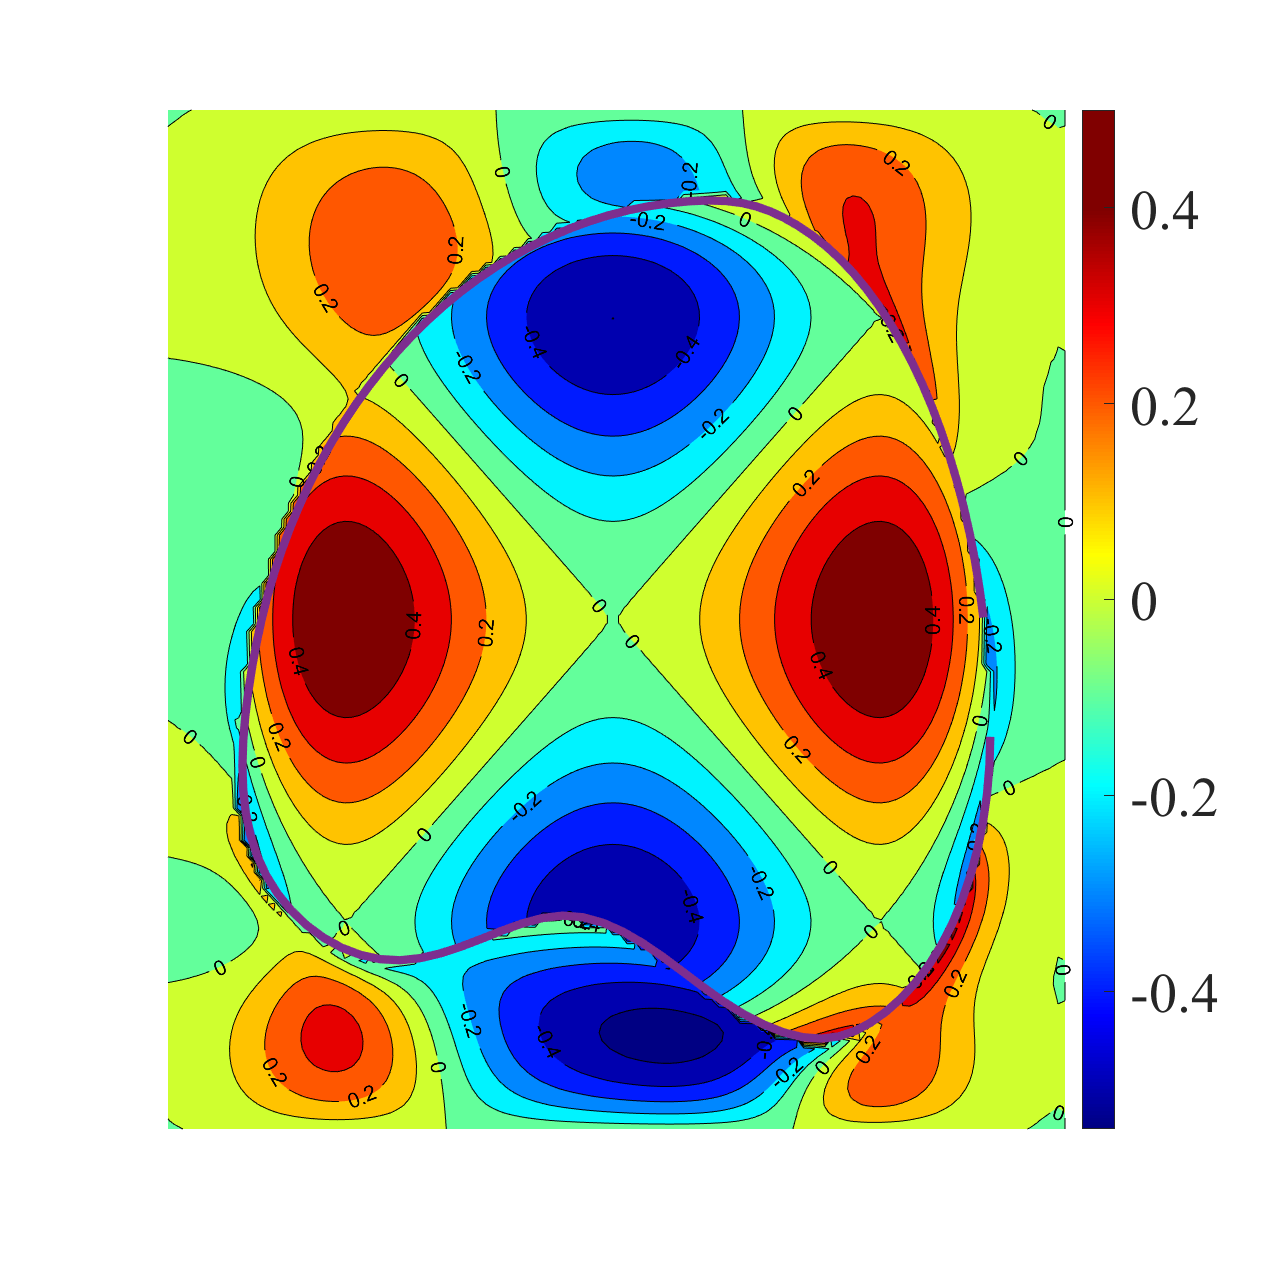
\includegraphics[width=0.3\textwidth]{figure/figure_v1.eps}}
    \subfigure[The velocity field $u^{(2)}$]{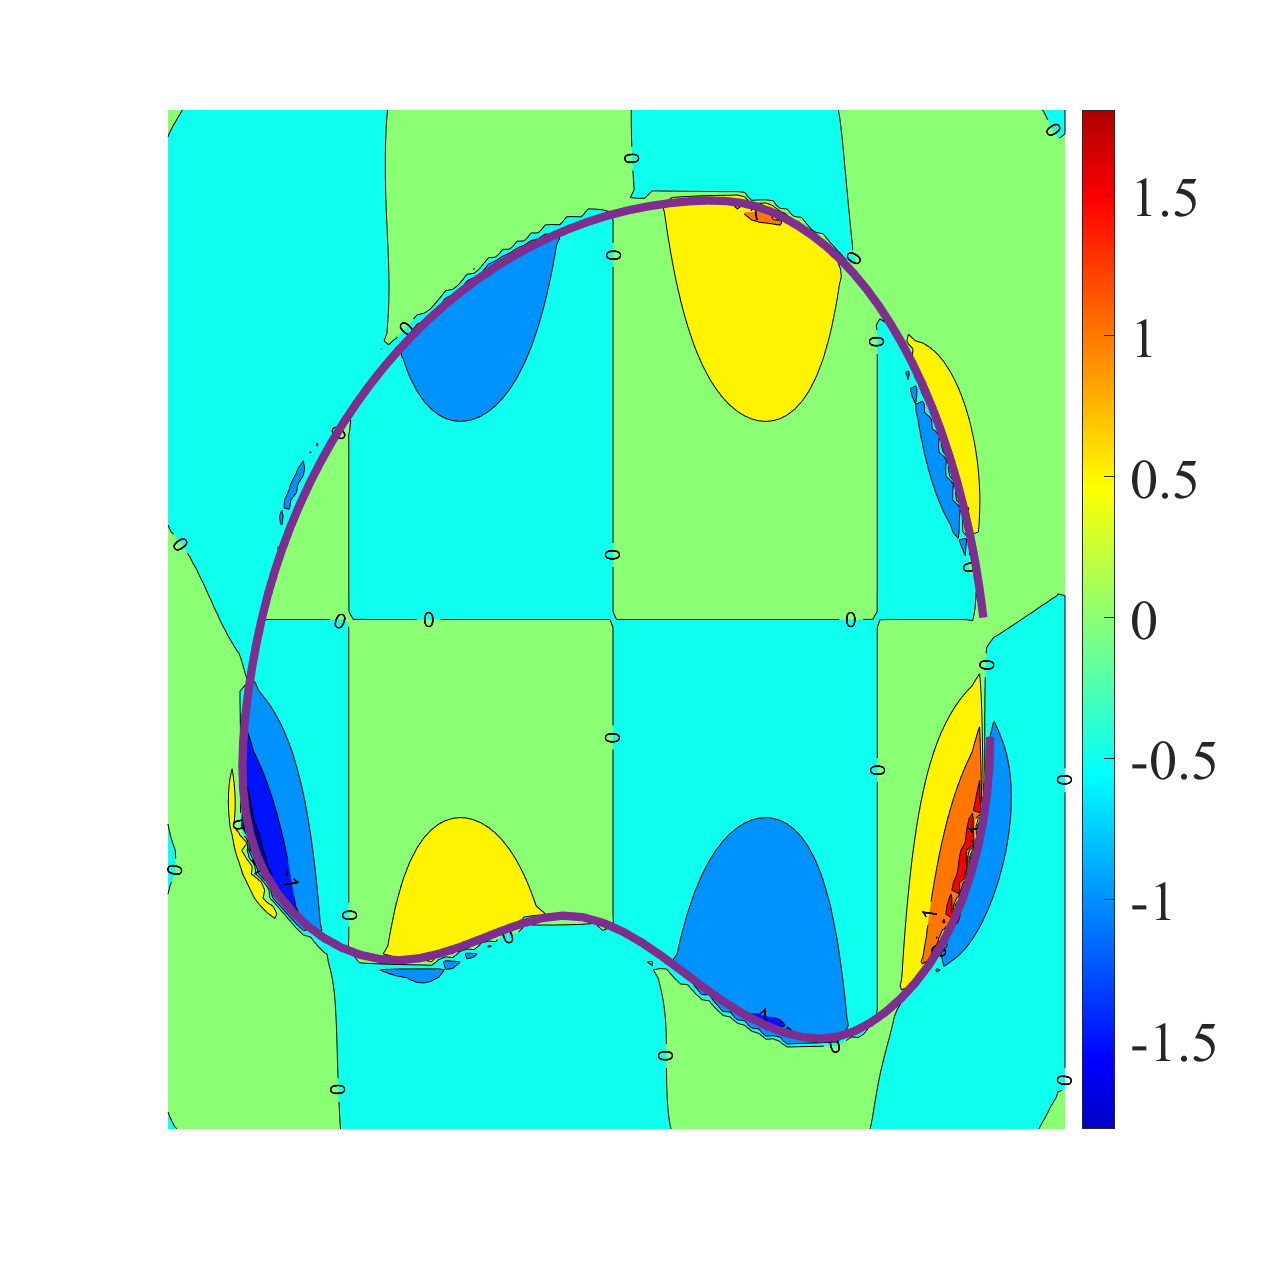
\includegraphics[width=0.3\textwidth]{figure/figure_v2.eps}}
    \subfigure[The pressure field $p$]{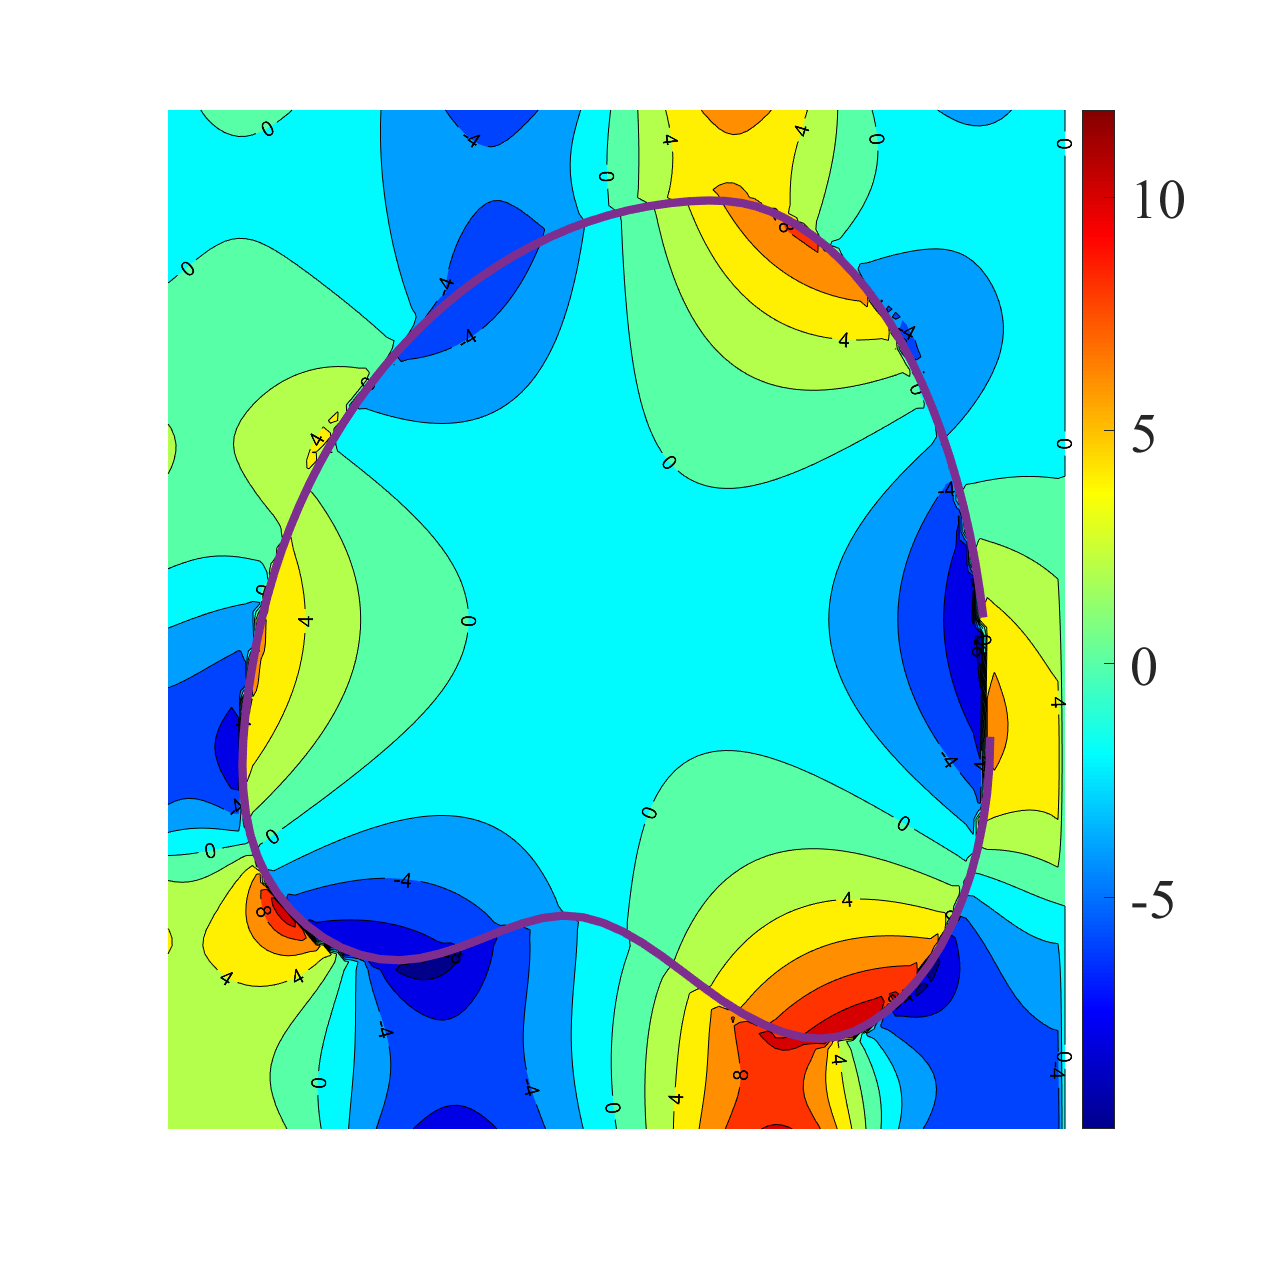
\includegraphics[width=0.3\textwidth]{figure/figure_q.eps}}
    \caption{The numerical solutions  for example 2 on the $512 \times 512$ grid.}
    \label{Stokes2D}
\end{figure}

\textbf{Example 3.}
 This example solves the Gray-Scott model which consists of two singularly perturbed reaction-diffusion equations given by
$$
\begin{aligned}
&u_{t}=\epsilon_{1} \Delta u+\frac{1}{\epsilon_{0}}\left[\gamma(1-u)-u v^{2}\right] \\
&v_{t}=\epsilon_{2} \Delta v+\frac{1}{\epsilon_{0}}\left[u v^{2}-(\gamma+\kappa) v\right]
\end{aligned}
$$

Here, $u=u(x, y, t)$ and $v=v(x, y, t)$ are two unknown smooth functions, describing the concentration of some chemical substances in a bounded domain $\Omega$ for $t \geqslant 0 ; \gamma$ and $\kappa$ are respectively the feed and removal rate; $\epsilon_{0}, \epsilon_{1}$ and $\epsilon_{2}$ are small reactive or diffusive coefficients. In this example, the model is assumed to satisfy the homogeneous Neumann boundary condition that $\partial_{\mathrm{n}} u=\partial_{\mathrm{n}} v=0$ on $\partial \Omega$, initial condition and the involved parameters are specified as follows
$$
\begin{aligned}
&v(x, y, 0)=\left\{\begin{array}{cc}
\frac{1}{4} \sin ^{2}(4 \pi x) \sin ^{2}(4 \pi y), & -0.25 \leqslant x, y \leqslant 0.25 \\
0, & \text { others. }
\end{array}\right. \\
&u(x, y, 0)=1-2 v(x, y, 0) \\
&\gamma=0.024, \kappa=0.06, \epsilon_{0}=0.01, \epsilon_{1}=0.008, \epsilon_{2}=0.004
\end{aligned}
$$

The bounding box $\mathcal{B}$ for the interface problem is set to be $\mathcal{B}=(-2.0,2.0) \times(-2.0,2.0)$ and the tolerance is $10^{-8}$. Time direction is discretized by the second-order Strang splitting method\cite{MacNamara2016}. The numerical results when $T = 1,2,7,11,17,21,25,50$ are plotted in Fig.\,\ref{PKFBIRD}. Tab.\,\ref{tab:PKFBIRD} we present the execution time on the CPU and GPU of the parallel algorithm for different 
computing scales, In order to verify the computational efficiency and stability, the GPU acceleration ratio and numerical accuracy are also shown in the table. It is calculated selecting four different problem sizes: $128 \times 128$,  $256 \times 256$, $512 \times 512$, $1024 \times 1024$, the time step is increasing with the increase of the grid size. From the table we can see that the GPU acceleration ratio increases with increasing of the computation scale, It can be seen that a better performance is obtained when large problems are considered, which means our parallel method scales well.
\begin{table}[htpt!]

\centering
\begin{tabular}{c|ccccc}
\hline  boundary condition & \text { grid size }  & $128 \times 128$ & $256 \times 256$ & $512 \times 512$ &  $1024 \times 1024$\\
  &\text {Time steps}& $ 8$ & 16 & 32 &  64 \\
\hline Neumann & \text {CPU time}& $1.21 \mathrm{~s}$ & $ 8.98 \mathrm{~s}$ & $74.97 \mathrm{~s}$ & $633.78\mathrm{~s}$ \\

 & GPU time & $0.40 \mathrm{~s}$ & $1.04 \mathrm{~s}$ & $3.29 \mathrm{~s}$ & $12.07\mathrm{~s}$  \\
  & Speedup & $3.0250$ & $8.6346$ & $22.7872$ & $52.5086
$  \\
\hline
\end{tabular}
            \caption{Simulation time of CPU-based and GPU-based KFBI method, as well as the speedup  achieved by  GPU-based
 solver over the CPU-based solver. }
            \label{tab:PKFBIRD}
\end{table}
\begin{figure}[ht]
    \centering{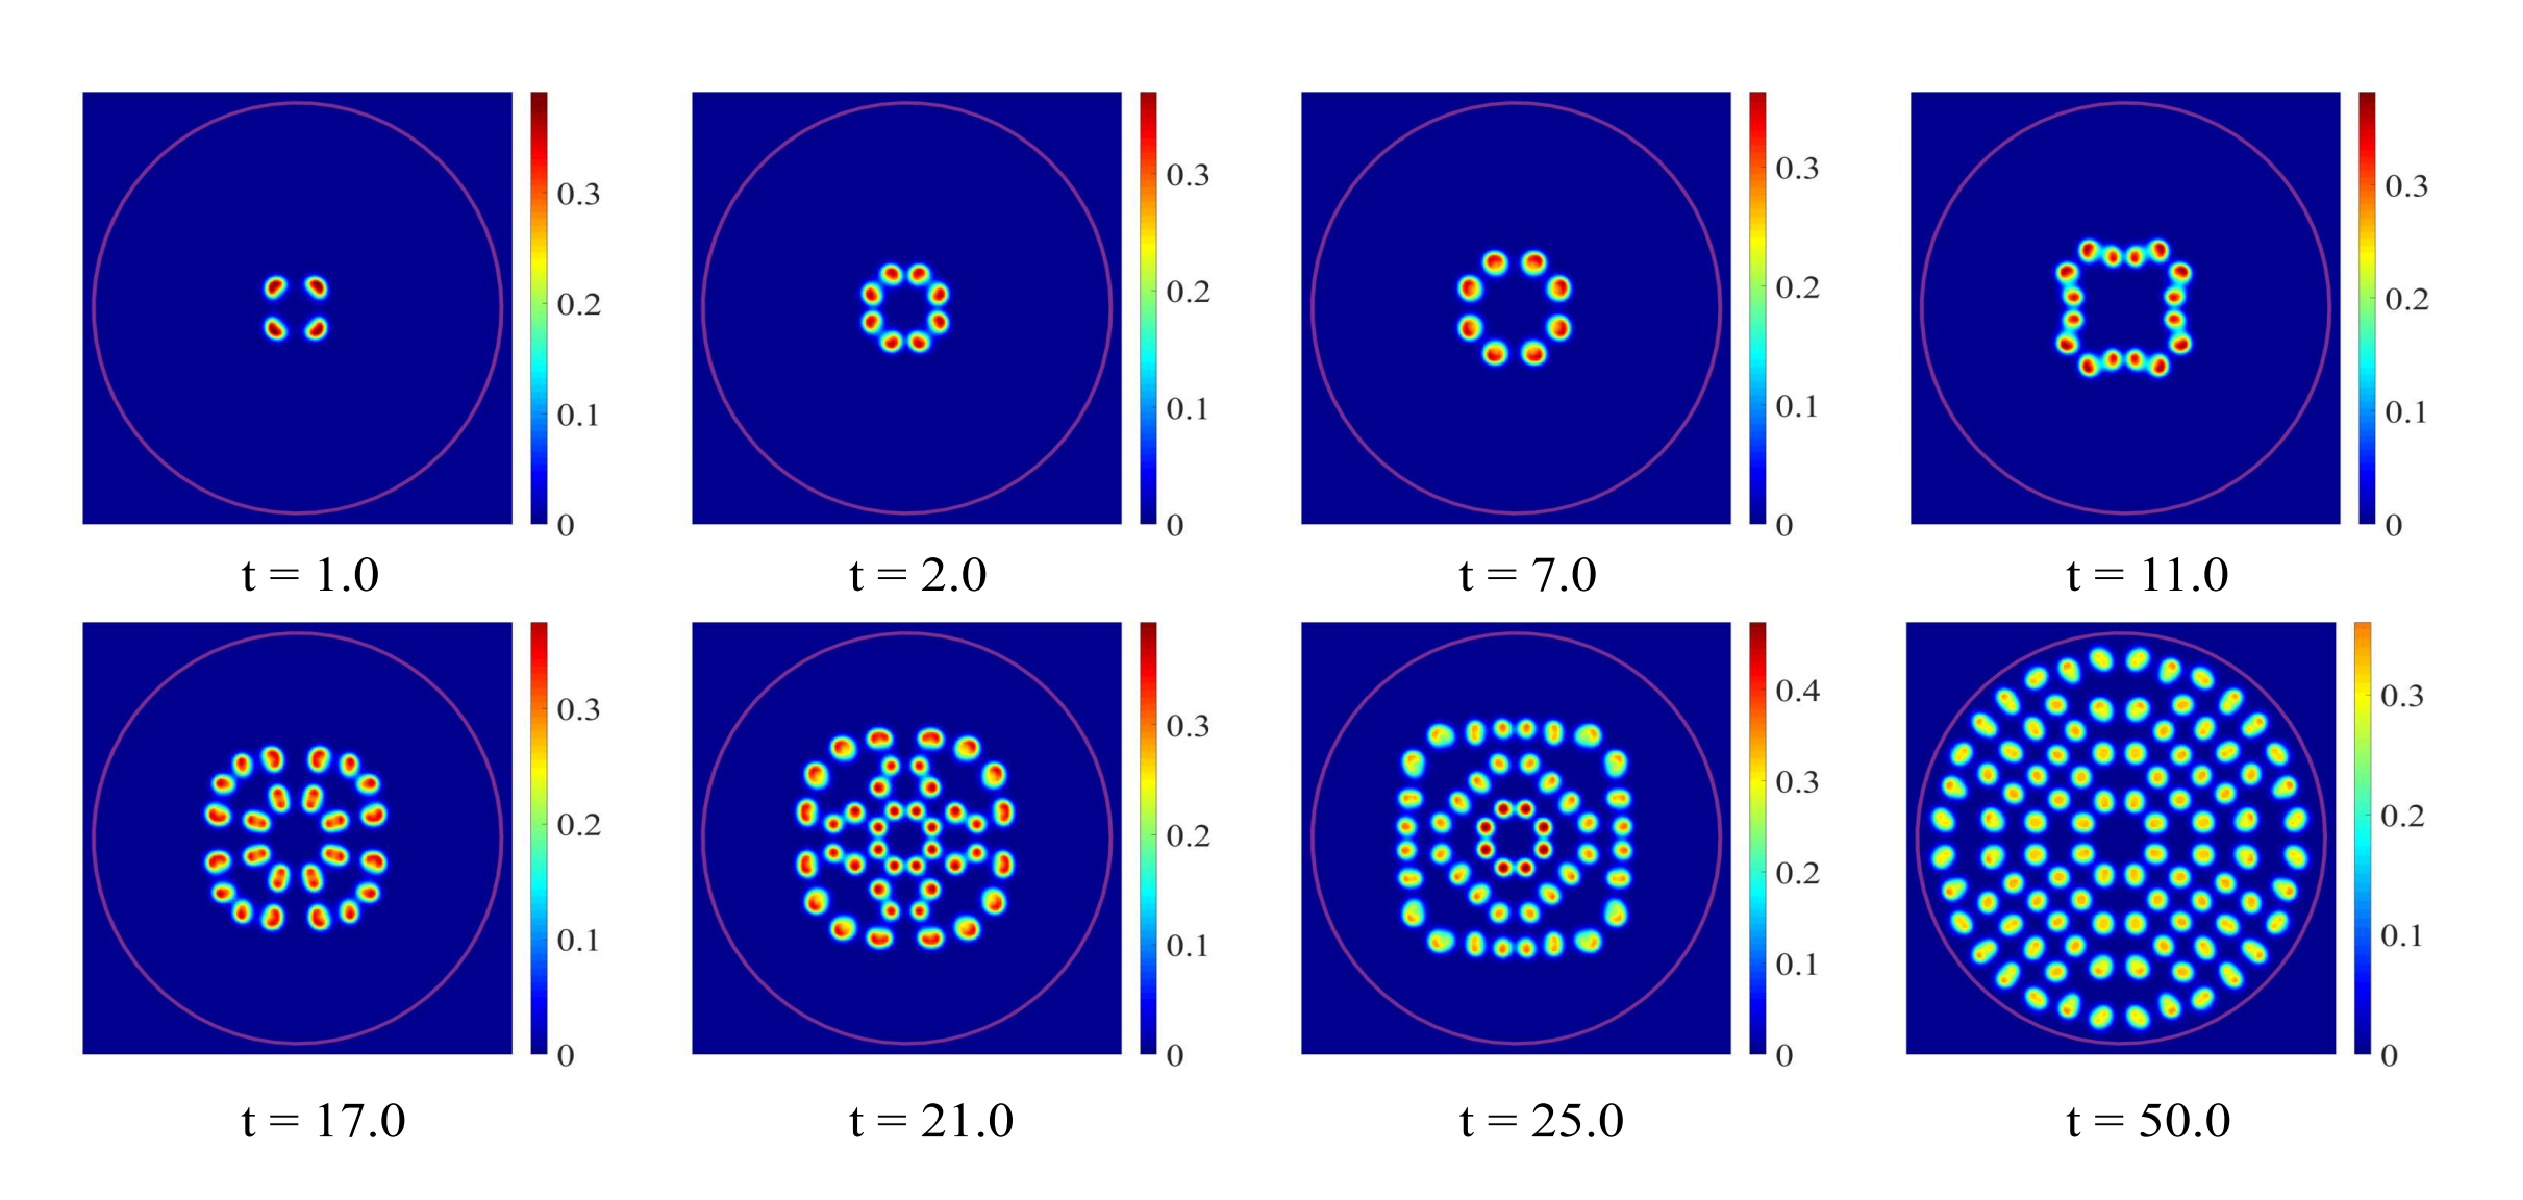
\includegraphics[width=1.0\textwidth]{figure/DFN2_new.eps}}
    \caption{the radius $r = 1.8$, $T = 1,2,7,11,17,21,25,50$ on the $128 \times 128$ grid.The bounding box $\mathcal{B}$  is set to be $\mathcal{B}=(-2.0,2.0) \times(-2.0,2.0)$ .}
    \label{PKFBIRD}
\end{figure}

\iffalse
% \textbf{Example 4.Laplace equation in 3D torus domain}
% \begin{table}[H]
% \centering
% \begin{tabular}{c|c|ccccc}
% \hline Boundary & \text { grid size }  & $32^3$ & $64^3$ & $128^3$ &  $256^3$ & $512^3$\\
% \hline & \text {CPU time}& $0.64 \mathrm{~s}$ & $3.03 \mathrm{~s}$ & $21.87 \mathrm{~s}$ & $158.91\mathrm{~s}$ & $1654.21\mathrm{~s}$\\
% Dirichlet & GPU time&$0.56 \mathrm{~s}$ & $0.59 \mathrm{~s}$ & $0.68 \mathrm{~s}$ & $1.26\mathrm{~s}$  & $3.98 \mathrm{~s}$ \\
% &\left\|\mathbf{e}_{h}\right\|_{\infty} & 7.5 \mathrm{E}-4 & 1.0 \mathrm{E}-4 & 1.6 \mathrm{E}-5 &2.1  \mathrm{E}-6&3.2  \mathrm{E}-7 \\
% \hline
% \end{tabular}
%     \caption{\footnotesize{DBVP of the Laplace equation in torus domain with  bounding box $\mathcal{B}=(0,1.2) \times(0,1.2)\times(0,1.2)$.}}
%     \label{tab:my_label}
% \end{table}

% \begin{figure}[H]
%     \centering{\includegraphics[width=0.45\textwidth]{figure/3D.png}}
%     \caption{\footnotesize{The numerical solutions with the $256 \times 256 \times 256$ grid.}}
% \end{figure}
\fi
\textbf{Example 4.}
 This example solves the Dirichlet BVP of the Stokes equation on an sphere $\Omega$ which is given by
\begin{equation}
\Omega=\left\{(x, y, z) \in \mathbb{R}^3: \frac{x^2}{a^2}+\frac{y^2}{b^2}+\frac{z^2}{c^2}<1\right\}
\label{sphere}
\end{equation}
with $a=1.0, b=0.8, c=0.6$.  The bounding box $\mathcal{B}$ for the interface problem is $\mathcal{B}=[-1.2,1.2] \times[-1.2,1.2] \times[-1.2,1.2]$.   The Dirichlet BC is chosen so that the exact solution reads
% \begin{equation}
% \begin{aligned}
% & u^{(1)}(x, y, z)= \begin{cases}\exp (\cos y)+\exp (\sin z), & x^2+y^2+z^2>1, \\
% -4\left(1-x^2-y^2\right) x y-4 x^2 z^2+\left(x^2+3 z^2-2\right)\left(z^2-x^2\right), & x^2+y^2+z^2 \leq 1,\end{cases} \\
% & u^{(2)}(x, y, z)= \begin{cases}\exp (\sin x), & x^2+y^2+z^2>1, \\
% -4 x^2 y^2+\left(3 x^2+y^2-2\right)\left(x^2-y^2\right), & x^2+y^2+z^2 \leq 1,\end{cases} \\
% & u^{(3)}(x, y, z)= \begin{cases}\exp (\cos (x)), & x^2+y^2+z^2>1, \\
% -4\left(1-x^2-z^2\right) x z, & x^2+y^2+z^2 \leq 1\end{cases} \\
% & p(x, y, z)= \begin{cases}\exp (\cos x+\sin y)+\exp (\cos z+\sin x), & x^2+y^2+z^2>1, \\
% (x-1)^3+(y-1)^3+(z-1)^2, & x^2+y^2+z^2 \leq 1 .\end{cases} \\
% &
% \end{aligned}
% \end{equation}
\begin{equation}
\begin{aligned}
& u^{(1)}(x, y, z)= \exp (\cos y)+\exp (\sin z)-4\left(1-x^2-y^2\right) x y-4 x^2 z^2+\left(x^2+3 z^2-2\right)\left(z^2-x^2\right) \\
& u^{(2)}(x, y, z)= \exp (\sin x)-4 x^2 y^2+\left(3 x^2+y^2-2\right)\left(x^2-y^2\right)\\
& u^{(3)}(x, y, z)= \exp (\cos (x))-4\left(1-x^2-z^2\right) x z \\
& p(x, y, z)= \exp (\cos x+\sin y)+\exp (\cos z+\sin x)+8  (3  x^2 - y^2)  y + 8  x  (3  z^2 - x^2) \\
&
\end{aligned}
\end{equation}


The error orders and execution times on the CPU and GPU are encapsulated in Table \ref{tab:Stokes3D}, derived from four distinct problem sizes: $32^3$,  $64^3$, $128^3$, $256^3$, and $512^3$. The table reveals an increasing GPU acceleration ratio with the escalation of computational scale. It is observed that enhanced performance is achieved for larger problems, indicating the scalability of the parallel method.
\begin{table}[H]
\centering
\begin{tabular}{c|c|ccccc}
\hline Boundary & \text { grid size }  & $32^3$ & $64^3$ & $128^3$ &  $256^3$ \\
\hline & \text {CPU time} & $44.85 \mathrm{~s}$ & $272.39 \mathrm{~s}$ & $1948.24\mathrm{~s}$ &$13521.36\mathrm{~s}$\\
Dirichlet & \text{GPU time} & $1.34 \mathrm{~s}$ & $2.82 \mathrm{~s}$ & $4.98\mathrm{~s}$  & $38.62 \mathrm{~s}$ \\
 & \text{Speedup} & $33.47$ & $96.59$ & $391.21$  & $350.11$ \\
%&\left\|\mathbf{e}_{h}\right\|_{\infty} &  5.69 \mathrm{E}-2 & 5.89 \mathrm{E}-3 &8.78  \mathrm{E}-4&1.04 \mathrm{E}-4 \\
\hline
\end{tabular}
    \caption{BVP of the Stokes equation  on the bounding box $\mathcal{B}=(-1.2,1.2) \times(-1.2,1.2)\times(-1.2,1.2)$ with GMRES iterition method.}
    \label{tab:Stokes3D}
\end{table}

% \begin{figure}[htb]
%     \centering
%     \subfigure[The velocity field $u^{(1)}$]{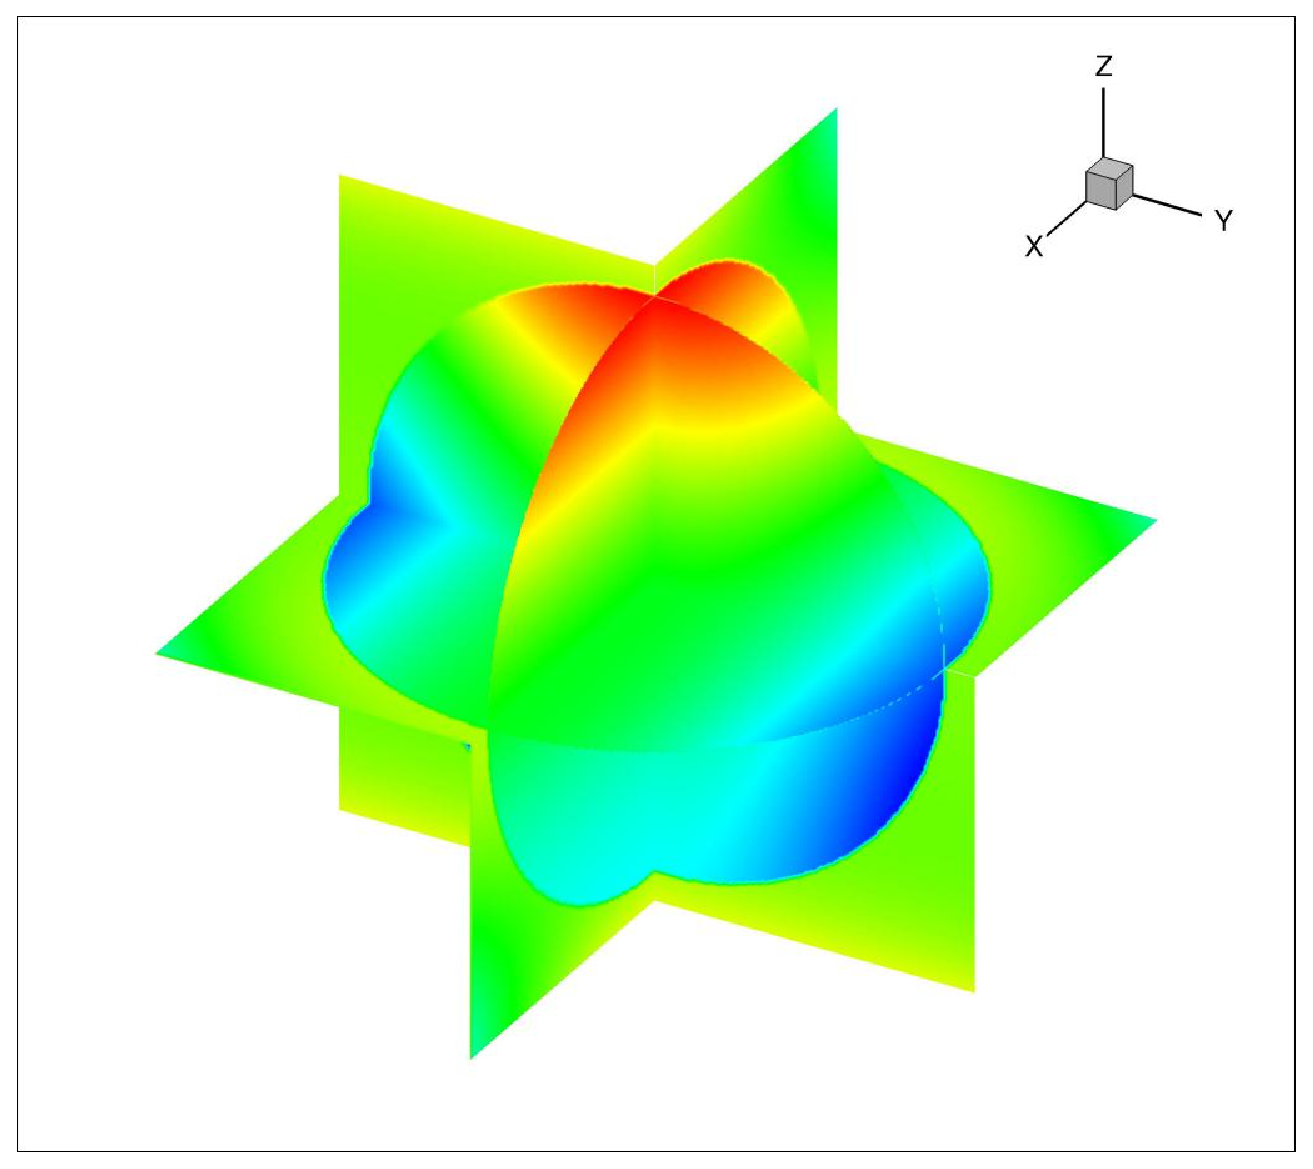
\includegraphics[width=0.4\textwidth]{figure/u1.eps}}
%     \subfigure[The velocity field $u^{(2)}$]{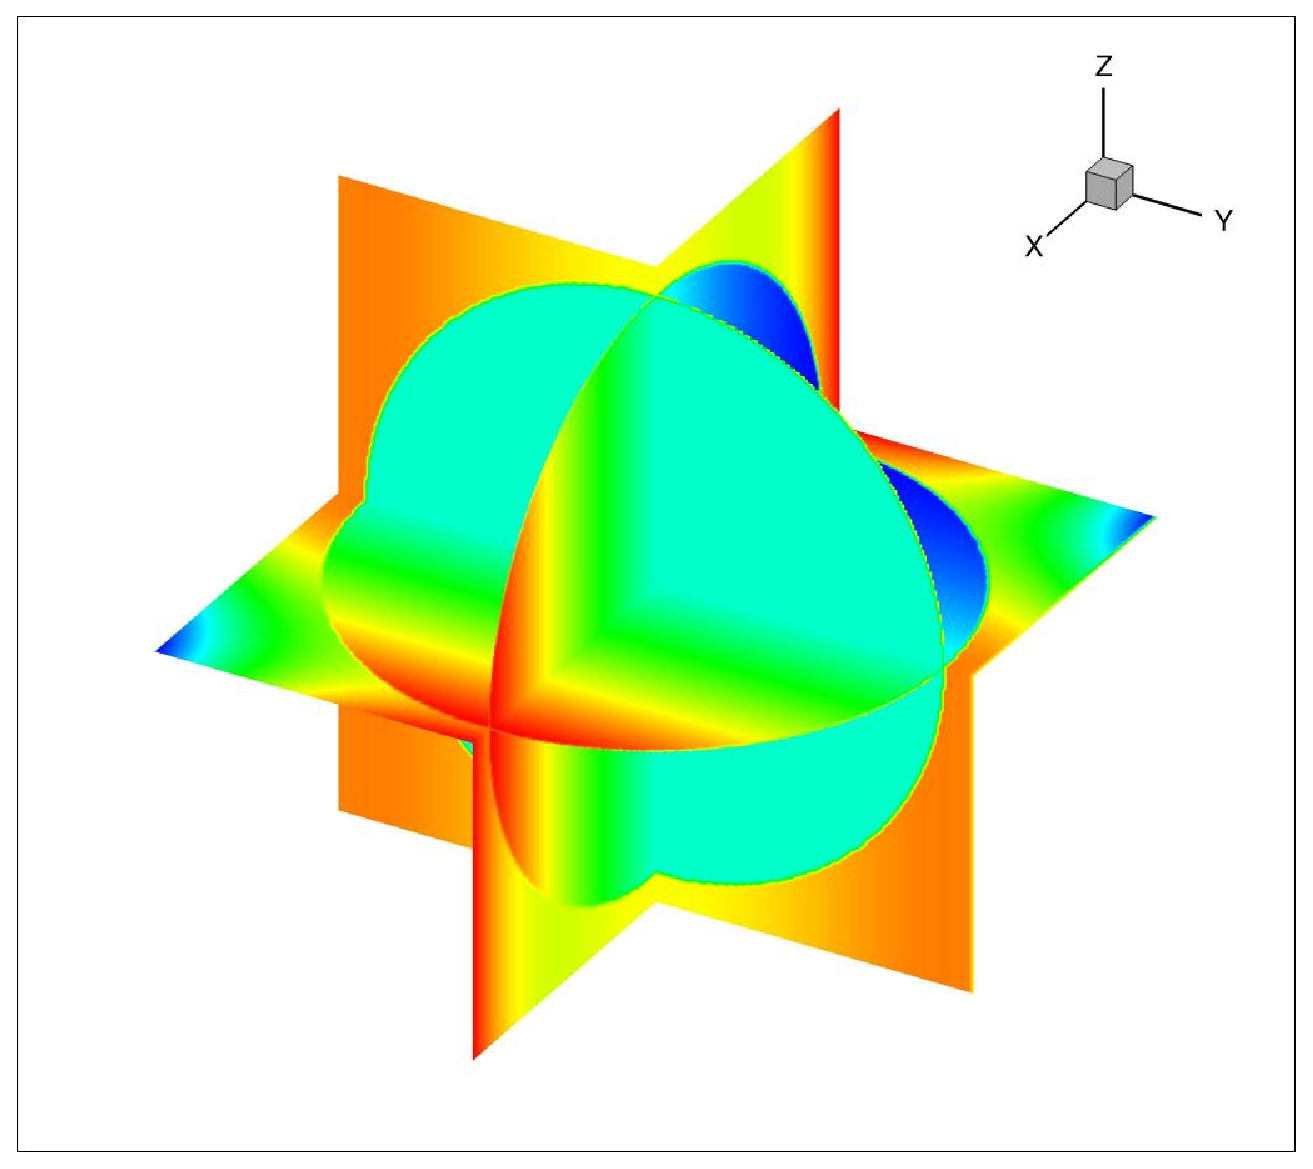
\includegraphics[width=0.4\textwidth]{figure/u2.eps}}
%     \subfigure[The velocity field $u^{(3)}$]{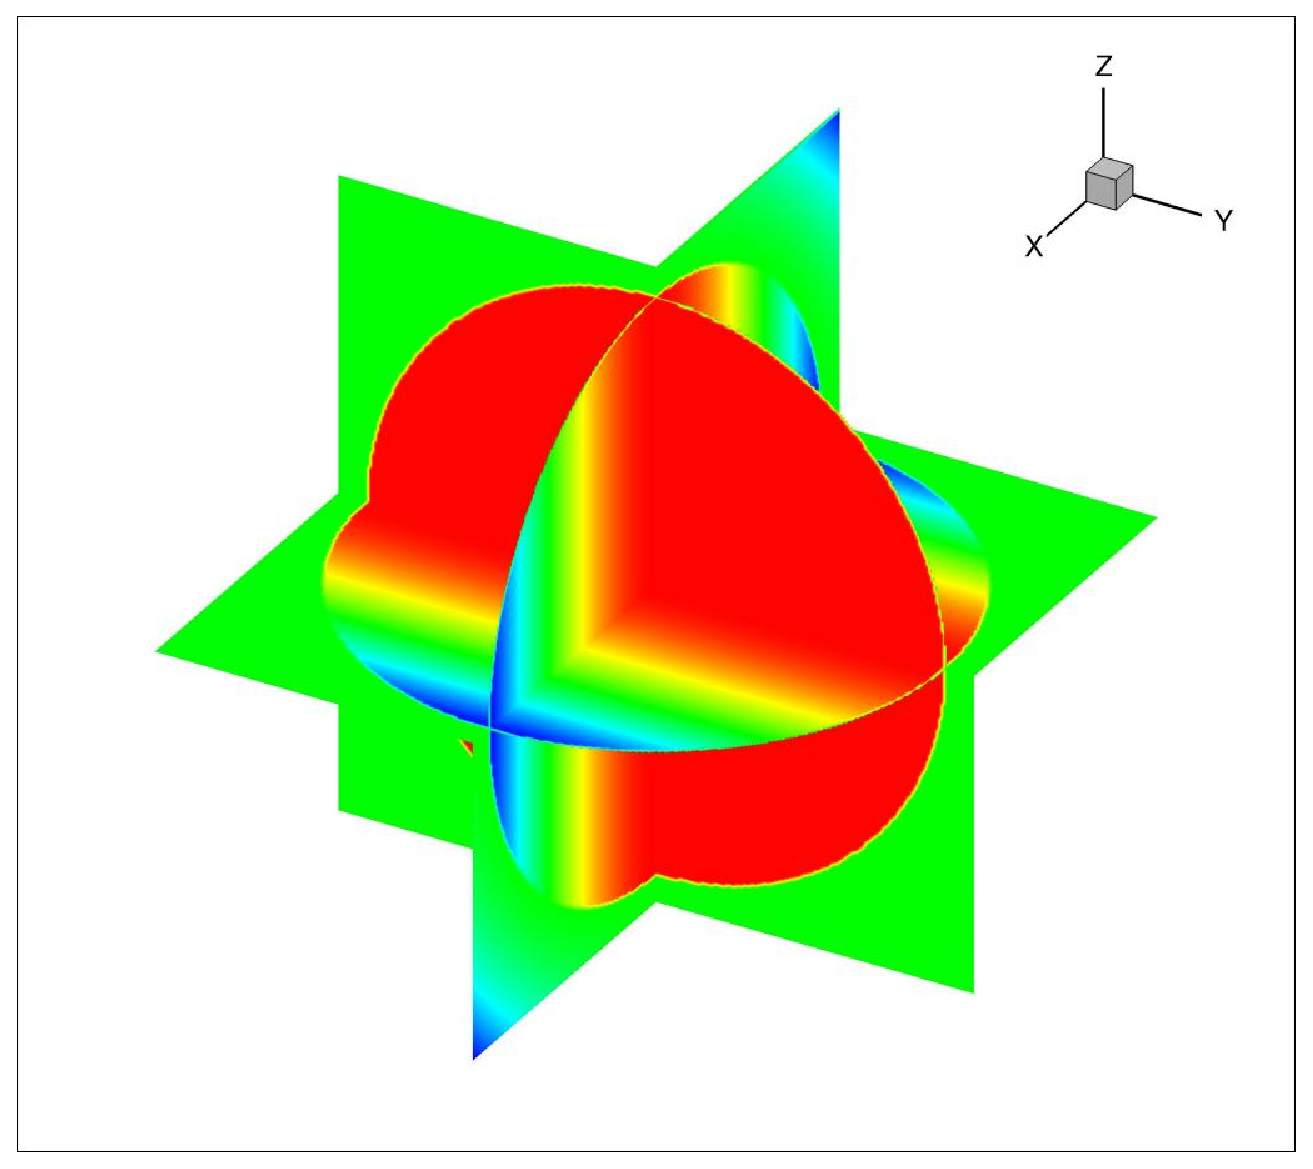
\includegraphics[width=0.4\textwidth]{figure/u3.eps}}
%     \subfigure[The pressure field $p$]{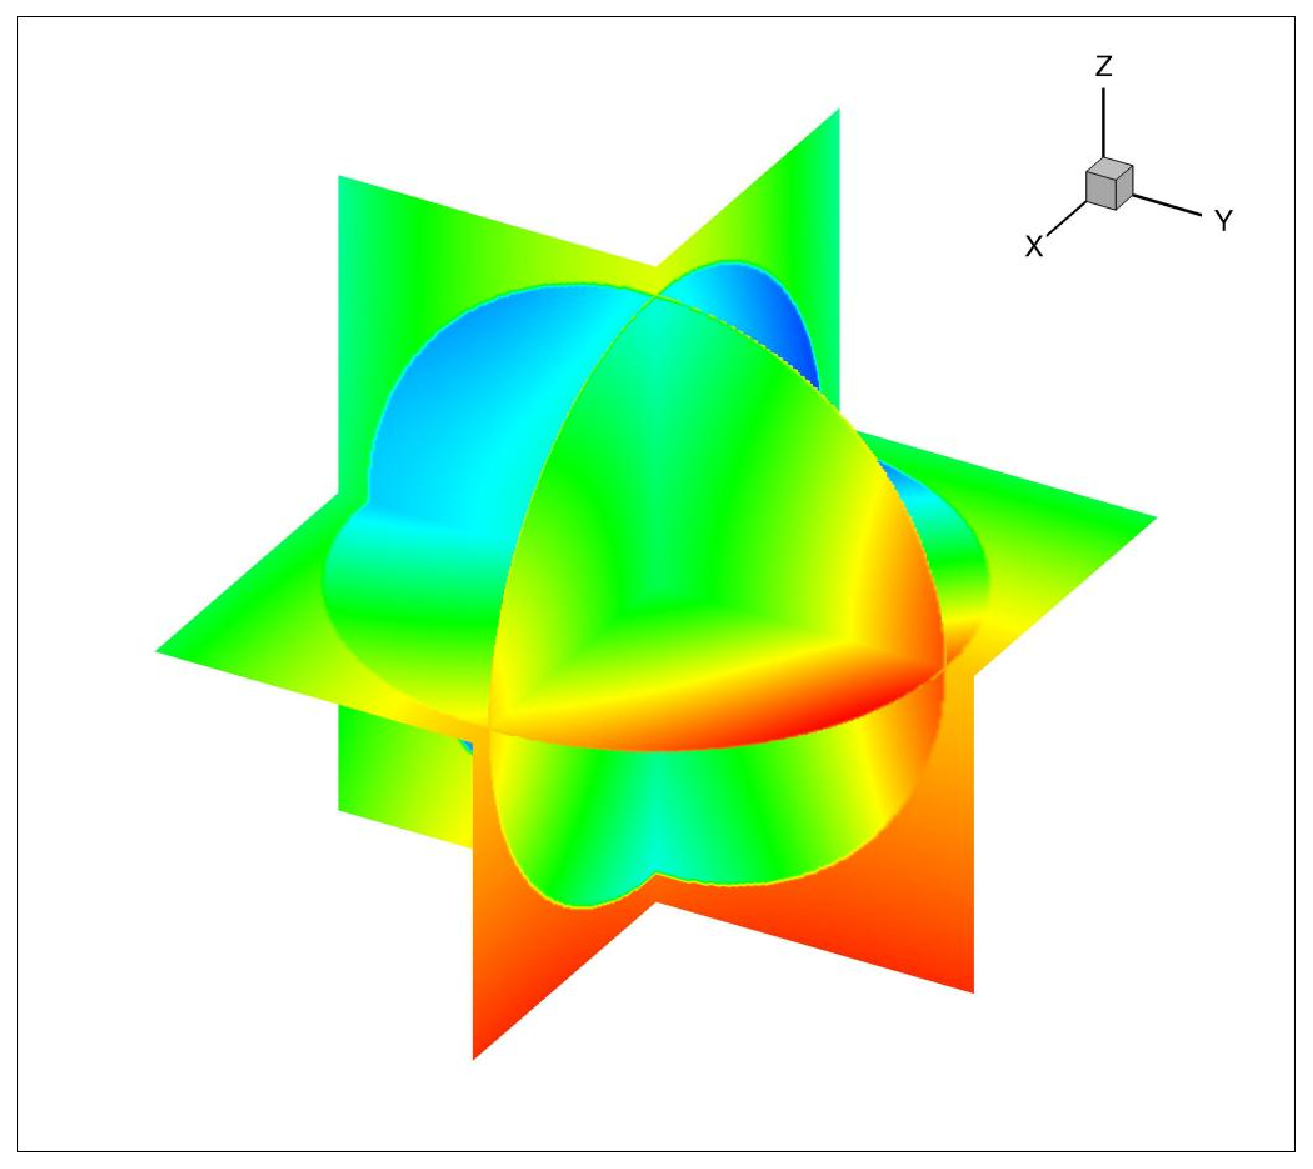
\includegraphics[width=0.4\textwidth]{figure/p.eps}}
%     \caption{The numerical solutions  for example 5 on the $128 \times 128 \times 128$ grid.}
%     \label{Stokes3D}
% \end{figure}
\begin{figure}[htpt!]
    \centering{\includegraphics[width=1.05\textwidth]{figure/3D2.eps}}
    %\caption{The numerical solutions for feature edge in example 5 on the $128 \times 128 \times 128$ grid.}
    \label{One_Poisson}
\end{figure}


\subsection{Multiple-GPU results}
To augment computational precision, refinement
is applied to the computational grid. Example 6 uses the same numerical test cases as examples 1, 3, and 4. Table \ref{tab:multi_gpu} displays the computation times for solving the 2D Laplace, reaction-diffusion, and 3D Stokes equation. These computations were executed using 1, 2, 4, and 8 GPUs.

In the Fig.\,\ref{MULTIGPU}, we can conclude that multi-GPUs parallel computing achieves linear speedup, despite a slight decrease in single-GPU performance when more GPUs are employed, as shown in Tab.\,\ref{tab:multi_gpu}. The linear growth of parallel efficiency hindrance can be attributed to inter-GPU communication, involving tasks such as the distribution of boundary data(point 1 of procedure 2), exchange of ghost cell data(points 3 and 4 of procedure 2), and collection of boundary data(the point 6 of procedure 2) in \ref{Sec:Algorthm summary}.


\begin{table}[H]
\centering
\footnotesize
\scalebox{0.8}{
\begin{tabular}{c|ccc|ccc|ccc}
\hline \text { equation } & & 2D Laplace && &2D reaction-diffusion &&& 3D Stokes&\\
\hline  \text {grid size }  & $4096^2$ & $8192^2$ & $16384^2$ & $4096^2$ & $8192^2$ & $16384^2$&$128^3$ &  $256^3$ &  $512^3$ \\
\hline $1$GPU & $0.25 \mathrm{~s}$ & $1.02 \mathrm{~s}$ &  &  $26.87 \mathrm{~s}$ & $106.51 \mathrm{~s}$   &  & $4.98\mathrm{~s}$ &$38.62\mathrm{~s}$ \\
   $2$GPUs  & $0.15 \mathrm{~s}$ & $0.51 \mathrm{~s}$&& $13.74 \mathrm{~s}$ & $53.87 \mathrm{~s}$ & & $2.72 \mathrm{~s}$ & $19.56 \mathrm{~s}$\\
    $4$GPUs   & $0.09 \mathrm{~s}$ & $0.28 \mathrm{~s}$&$1.01 \mathrm{~s}$& $9.05 \mathrm{~s}$ & $27.12 \mathrm{~s}$ &$123.78 \mathrm{~s}$  &  $2.16 \mathrm{~s}$ &  $11.8 \mathrm{~s}$  \\
      $8$GPUs   & $0.06 \mathrm{~s}$ & $0.18 \mathrm{~s}$&$0.62 \mathrm{~s}$& $7.58 \mathrm{~s}$ & $20.38 \mathrm{~s}$ & $74.93\mathrm{~s}$ &  $2.05 \mathrm{~s}$ &  $9.16 \mathrm{~s}$ &$66.21 \mathrm{~s}$ \\
      
\hline
\end{tabular}
}
    \caption{Multi-GPUs execution time vs. single GPU.}
    \label{tab:multi_gpu}
\end{table}

\begin{figure}[htb]
    \centering
    \subfigure[2D Laplace]{\includegraphics[width=0.31\textwidth]{figure/threadsperblockm.eps}}
    \subfigure[2D reaction-diffusion]{\includegraphics[width=0.31\textwidth]{figure/threadsperblockm_standard.eps}}
    \subfigure[3D Stokes]{\includegraphics[width=0.31\textwidth]{figure/threadsperblockm_standard2.eps}}
    \caption{Comparison of parallel efficiency with different numbers of GPUs}
    \label{MULTIGPU}
\end{figure}

